A trusted revision can withdraw progress whose computation remains
valid. In streaming speech correction, selected corrections feed later
recognition~\cite{vu2026streamcorrect}; trusted feedback means acceptance
by the original protected selection process. We call the loss of a
still-supported whole view an \emph{avoidable withdrawal}. In
Figure~\ref{fig:continuity_case}(a), display within two seconds (D2) and
certified coverage within eight seconds (C8) both meet their deadlines,
yet the view becomes unavailable for 2.176~s.

\begin{figure*}[t]
\centering
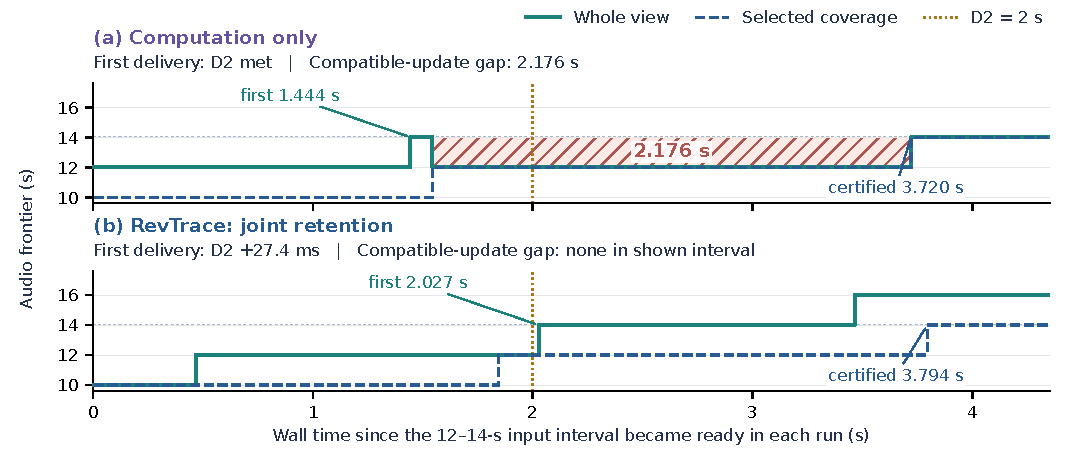
\includegraphics[width=\textwidth]{figures/timely_full_interval_case.pdf}
\caption{On-time delivery does not guarantee continued availability.
Two actual c16-overload runs process the same complete 12--14-s audio
interval using their own ready clocks. (a) Computation-only displays 37
new code points at 1.444~s, withdraws the supported view at 1.544~s and
restores identical text at 3.720~s. (b) RevTrace first displays the same
text at 2.027~s, 27.4~ms after D2, and maintains coverage; its 3.794-s
selected update retains an ahead 16-s view. Both certified deliveries
meet C8 (8~s). The dotted line marks D2 (2~s). These separate executions
have different interleavings; they are not an event-matched counterfactual.}
\label{fig:continuity_case}
\end{figure*}

First delivery is a past event; a consumer reads the current view.
Figure~\ref{fig:continuity_case}(a) exposes a service gap without a
corresponding refutation; Figure~\ref{fig:continuity_case}(b) preserves
the shown coverage but misses D2 by 27.4~ms. We therefore evaluate
continued availability separately from first delivery.

A dependable revision service must reject invalid uses while preserving
still-valid progress. When a whole view covers audio through 14~s,
installing a compatible 12-s state need not erase its supported 12--14-s
progress. A snapshot replacement does. A conservative version rule may
discard usable work, while retaining computation alone does not stop the
Consumer overwriting its supported ahead view. In a predeclared 24-speaker stratum,
computation retention improves timely audio coverage while increasing
backward movements of the displayed audio frontier, or \emph{frontier
withdrawals}, from 12 to 17. Coordinating computation and view retention
yields zero. RevTrace connects valid execution to continued availability
at the actual Consumer without changing which original result is selected.

The challenge is to act on evidence that arrives at different times.
A revision can remove a view's support without refuting the unresolved
input of a future call; confirming an input does not endorse the call's
own predicted successor. Thus one revision can require different actions
for an executing call, an accepted result and a displayed hypothesis.
RevTrace therefore checks complete-call input eligibility [EL], original
content-selection authority [AU], and whole-view support [SUP] separately
(Figure~\ref{fig:protocol}). Producer exit can end new-message admission
while an already accepted result remains eligible. A birth version,
matching text, or producer-liveness bit cannot stand in for these decisions.

Dependency reuse and revocation have established foundations in
incremental dialogue and computation
\cite{schlangen2011incremental,hammer2014adapton,hammer2015names}.
SSBD coordinates draft reuse with display masking~\cite{zeng2026ssbd};
PredGen speculates across evolving speech stages~\cite{li2025predgen}.
RevTrace realizes coordination around a recursively selected feedback
task: complete calls retain the original correction and update, while
the actual whole view is checked independently at selected-state
installation, binding reuse to the unchanged recursive task.

We make three contributions:
\begin{itemize}
\item A service contract exposing avoidable withdrawal and sufficient,
  executable witnesses for complete-call eligibility and whole-view
  support across trusted revisions
  (Sections~\ref{sec:contract}--\ref{sec:continuation}).
\item A joint coordinator that preserves the original selected transition
  relation while retaining eligible calls and supported whole views.
  Its conditional selected-trace argument connects early execution,
  durable selection and supported process failures
  (Sections~\ref{sec:continuation}--\ref{sec:protocol}).
\item Evidence that computation retention alone can worsen delivered
  progress, and that confirmed full calls improve timely service while
  preserving the selected task. Across eight previously unused native
  speakers, coverage increases by 53.3 percentage points
  (paired-speaker 95\% CI [44.8, 59.6]), with positive paired gains for all
  eight sources (Section~\ref{sec:eval}).
\end{itemize}

